% ================= CHAPTER 3 =================
\chapter{Methodology}
\vspace{0.5cm}
\minitoc
\vspace{1cm}

% ── Introduction (unnumbered) ────────────────────────────────────────────────
\section*{Introduction}
\addcontentsline{toc}{section}{Introduction}

This chapter presents the complete methodology of the PhishShield project, describing every step from dataset preparation to model training, explainability, robustness evaluation, and deployment. We begin by presenting the CRISP-DM framework that structures our work. We then introduce the global system pipeline and describe in detail the PhishFOE dataset used for model training. We subsequently explain all data preprocessing steps, specify the architectures and hyperparameters of the six trained models, and describe the XAI, adversarial robustness, and statistical validation strategies. Every design choice is grounded in the analysis presented in the preceding chapters.

% ── 3.1 CRISP-DM ─────────────────────────────────────────────────────────────
\section{Adopted Methodology: CRISP-DM}

Our project follows the \textbf{CRISP-DM} (Cross-Industry Standard Process for Data Mining) methodology, a well-established and iterative framework for applied machine learning projects. As illustrated in Figure~\ref{fig:crispdm}, CRISP-DM consists of six interdependent phases applied throughout the project lifecycle:

\begin{enumerate}
    \item \textbf{Business Understanding:} We identified the operational requirements for a phishing detection system used by security analysts: the system must be accurate, explainable, and robust against adversarial manipulation. These requirements drove every subsequent design decision.

    \item \textbf{Data Understanding:} We explored the PhishFOE dataset (101,063 labeled URLs, 29 features) to understand the distribution of classes, the nature of each feature, and potential data quality issues. This phase confirmed that the dataset is clean and nearly balanced, eliminating the need for oversampling.

    \item \textbf{Data Preparation:} We applied a preprocessing pipeline consisting of missing value handling, non-numeric column removal, and StandardScaler normalization. For deep learning models (CNN, LSTM), input tensors were reshaped from 2D to 3D format $(n_{\text{samples}}, n_{\text{features}}, 1)$.

    \item \textbf{Modeling:} We trained six models: three tree-based ML classifiers (LightGBM, XGBoost, Random Forest) and three deep learning architectures (MLP, CNN, LSTM), all using the same stratified 80/20 train-test split and the same scaled feature set.

    \item \textbf{Evaluation:} We evaluated all models on five metrics (Accuracy, Precision, Recall, F1-Score, AUC-ROC), performed Bootstrap Confidence Interval estimation and one-way ANOVA statistical tests, applied SHAP/LIME/PFI explainability analysis, and measured robustness under FGSM and PGD adversarial attacks.

    \item \textbf{Deployment:} The best model (LightGBM) was serialized and deployed as a FastAPI REST API connected to a Next.js web dashboard, providing real-time phishing detection with XAI explanations.
\end{enumerate}

\begin{figure}[H]
    \centering
    \includegraphics[width=0.55\linewidth]{"../Pictures/Screenshots/Capture d'écran 2026-05-07 151547"}
    \caption{The six phases of the CRISP-DM methodology applied to the PhishShield project. The circular structure reflects the iterative nature of the process: results from the Evaluation phase can trigger a return to earlier phases (e.g., Data Preparation or Modeling) to improve the system.}
    \label{fig:crispdm}
\end{figure}

% ── 3.2 System Architecture ──────────────────────────────────────────────────
\section{System Architecture and Global Pipeline}

Before presenting the individual methodology steps, Figure~\ref{fig:pipeline} provides an overview of the complete PhishShield pipeline, from raw data ingestion to deployed web application. This architecture integrates seven sequential stages, each described in detail in the following sections.

\begin{figure}[H]
\centering
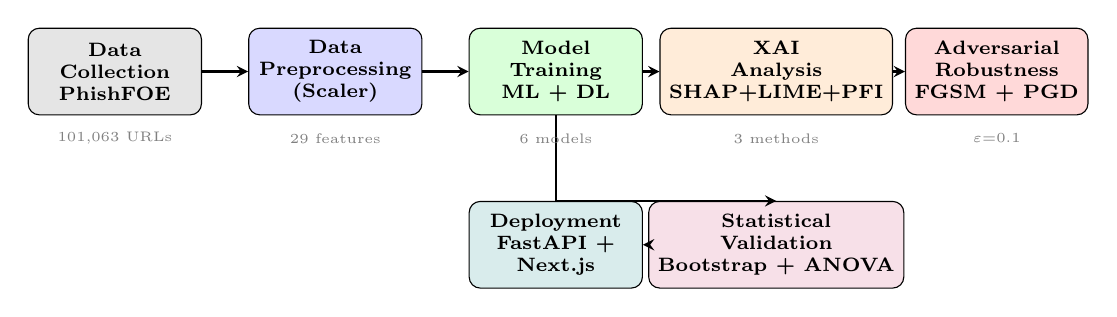
\begin{tikzpicture}[
    node distance=0.5cm,
    box/.style={rectangle, rounded corners=4pt, minimum width=2.2cm,
        minimum height=1.1cm, draw=black, align=center, font=\scriptsize\bfseries},
    arrow/.style={->, thick, >=stealth},
]

% Boxes
\node[box, fill=gray!20]   (d1) at (0,    0) {Data\\Collection\\PhishFOE};
\node[box, fill=blue!15]   (d2) at (2.8,  0) {Data\\Preprocessing\\(Scaler)};
\node[box, fill=green!15]  (d3) at (5.6,  0) {Model\\Training\\ML + DL};
\node[box, fill=orange!15] (d4) at (8.4,  0) {XAI\\Analysis\\SHAP+LIME+PFI};
\node[box, fill=red!15]    (d5) at (11.2, 0) {Adversarial\\Robustness\\FGSM + PGD};
\node[box, fill=purple!12] (d6) at (8.4, -2.2) {Statistical\\Validation\\Bootstrap + ANOVA};
\node[box, fill=teal!15]   (d7) at (5.6, -2.2) {Deployment\\FastAPI +\\Next.js};

% Horizontal arrows
\draw[arrow] (d1) -- (d2);
\draw[arrow] (d2) -- (d3);
\draw[arrow] (d3) -- (d4);
\draw[arrow] (d4) -- (d5);

% Vertical arrows
\draw[arrow] (d3.south) -- ++(0,-0.6) -- (d6.north -| d3) -- (d6.north);
\draw[arrow] (d6) -- (d7);

% Labels below main row
\node[font=\tiny, text=gray] at (0,    -0.85) {101,063 URLs};
\node[font=\tiny, text=gray] at (2.8,  -0.85) {29 features};
\node[font=\tiny, text=gray] at (5.6,  -0.85) {6 models};
\node[font=\tiny, text=gray] at (8.4,  -0.85) {3 methods};
\node[font=\tiny, text=gray] at (11.2, -0.85) {$\varepsilon$=0.1};

\end{tikzpicture}
\caption{Global architecture of the PhishShield system. The pipeline flows from data collection (grey) through preprocessing (blue), model training (green), XAI analysis (orange), and adversarial robustness testing (red). Statistical validation (purple) runs in parallel with training. The validated best model is then deployed (teal) as a production-ready web application.}
\label{fig:pipeline}
\end{figure}

% ── 3.3 Dataset Description ──────────────────────────────────────────────────
\section{Dataset Description}

\subsection{PhishFOE Dataset}

The primary dataset used in this project is \textbf{PhishFOE} \cite{phishfoe}, a recent and large-scale labeled dataset specifically designed for machine learning-based phishing detection. PhishFOE comprises \textbf{101,063 URLs}, each labeled as phishing (1) or legitimate (0), with 29 features extracted from two sources: the raw URL string and the HTML content of the corresponding web page.

The dataset presents several properties that motivated its selection as the primary training resource:

\begin{itemize}
    \item \textbf{Scale:} With over 100,000 labeled instances, PhishFOE provides sufficient training data for both gradient boosting and deep learning models without requiring data augmentation.
    \item \textbf{Feature richness:} The 29 features cover four complementary dimensions of phishing indicators, described in detail in Section~\ref{subsec:features}.
    \item \textbf{Balance:} The dataset is naturally near-balanced: 49,491 phishing URLs (49.0\%) and 51,572 legitimate URLs (51.0\%), eliminating the need for oversampling techniques such as SMOTE.
    \item \textbf{Data quality:} No missing values were detected across the 101,063 records.
\end{itemize}

\textit{Note on additional datasets:} In Chapter 4, we evaluate the generalization capability of all six trained models on three additional independent benchmark datasets (UCI Phishing Website dataset \cite{uci_phishing}, the Phishing Legitimate Full dataset \cite{phishing_leg}, and the dataset\_phishing benchmark \cite{ds_phishing}). These datasets are used exclusively for cross-dataset evaluation and are not involved in training or hyperparameter selection.

\subsection{Feature Description}
\label{subsec:features}

The 29 features used in this project are organized into four categories, as summarized in Table~\ref{tab:features}.

\begin{table}[H]
\caption{Description of the 29 features used in the PhishShield system}
\label{tab:features}
\vspace{4pt}
\centering
\begin{tabular}{|l|l|p{7cm}|}
\hline
\textbf{Category} & \textbf{Feature Name} & \textbf{Description} \\
\hline
\textit{Security} & IsHTTPS & 1 if the URL uses HTTPS, 0 otherwise \\
\textit{Security} & IsDomainIP & 1 if the domain is an IP address (phishing indicator) \\
\hline
\textit{URL Structure} & URLLength & Total number of characters in the URL \\
\textit{URL Structure} & NoOfSubDomain & Number of subdomain levels \\
\textit{URL Structure} & NoOfDots & Number of dot characters \\
\textit{URL Structure} & NoOfObfuscatedChar & Count of URL-encoded or obfuscated characters \\
\textit{URL Structure} & NoOfEqual & Number of ``='' characters in the URL \\
\textit{URL Structure} & NoOfQmark & Number of ``?'' characters \\
\textit{URL Structure} & NoOfAmp & Number of ``\&'' characters \\
\textit{URL Structure} & NoOfDigits & Number of digit characters in the URL \\
\hline
\textit{HTML Content} & LineLength & Average line length of the HTML source \\
\textit{HTML Content} & HasTitle & 1 if the page has a \texttt{<title>} tag \\
\textit{HTML Content} & HasMeta & 1 if the page has \texttt{<meta>} tags \\
\textit{HTML Content} & HasFavicon & 1 if the page loads a favicon \\
\textit{HTML Content} & HasExternalFormSubmit & 1 if forms submit to external domains \\
\hline
\textit{Phishing Signals} & HasCopyright & 1 if a copyright notice is present \\
\textit{Phishing Signals} & HasSocialNetworking & 1 if social network links are embedded \\
\textit{Phishing Signals} & HasPasswordField & 1 if the page contains a password input field \\
\textit{Phishing Signals} & HasSubmitButton & 1 if a submit button is present \\
\hline
\textit{Keywords} & HasKeywordBank & 1 if ``bank'' appears in URL or content \\
\textit{Keywords} & HasKeywordPay & 1 if ``pay'' appears in URL or content \\
\textit{Keywords} & HasKeywordCrypto & 1 if ``crypto'' appears in URL or content \\
\hline
\textit{Web Elements} & NoOfPopup & Number of popup windows triggered \\
\textit{Web Elements} & NoOfiFrame & Number of \texttt{<iframe>} elements \\
\textit{Web Elements} & NoOfImage & Number of \texttt{<img>} elements \\
\textit{Web Elements} & NoOfJS & Number of JavaScript files loaded \\
\textit{Web Elements} & NoOfCSS & Number of CSS files loaded \\
\textit{Web Elements} & NoOfURLRedirect & Number of URL redirections \\
\textit{Web Elements} & NoOfHyperlink & Total number of hyperlinks in the page \\
\hline
\end{tabular}
\end{table}

\subsection{Dataset Split}
\label{subsec:split}

The dataset was partitioned into a training set and a test set using a \textbf{stratified 80/20 split}:

\begin{itemize}
    \item \textbf{Training set:} 80,850 instances (80\%) — used to fit all ML and DL models.
    \item \textbf{Test set:} 20,213 instances (20\%) — used exclusively for performance evaluation.
\end{itemize}

Stratification ensures that the phishing-to-legitimate ratio is preserved identically in both subsets. A fixed \texttt{random\_state = 42} is used for reproducibility. The StandardScaler is fitted exclusively on the training set and applied to both training and test sets, preventing any data leakage from the test distribution into the normalization parameters.

% ── 3.4 Data Preprocessing ───────────────────────────────────────────────────
\section{Data Preprocessing}

Before feeding data to any model, a systematic preprocessing pipeline was applied to ensure data integrity and consistent representation across all experiments.

\subsection{Data Cleaning}

The raw PhishFOE CSV file was processed as follows:
\begin{itemize}
    \item Non-numeric columns (e.g., the raw URL string) were dropped, retaining only the 29 numeric features and the binary target label.
    \item Missing values were filled with zero (\texttt{fillna(0)}), as the rare missing entries corresponded to features that could not be extracted from the HTML (e.g., no favicon detected $\rightarrow$ 0).
    \item No duplicate rows were detected in PhishFOE; no deduplication was necessary.
\end{itemize}

\subsection{Class Distribution Analysis}

Figure~\ref{fig:classdist} presents the class distribution of the PhishFOE dataset after cleaning.

\begin{figure}[H]
    \centering
    \includegraphics[width=0.62\linewidth]{"../Pictures/Screenshots/Capture d'écran 2026-05-24 221810"}
    \caption{Class distribution of the PhishFOE dataset after preprocessing. The \textbf{blue bar} represents legitimate URLs (51,572 instances, 51.0\%) and the \textbf{orange bar} represents phishing URLs (49,491 instances, 49.0\%). The near-perfect balance between the two classes confirms that no oversampling (SMOTE) or undersampling is required for this dataset.}
    \label{fig:classdist}
\end{figure}

As visible in Figure~\ref{fig:classdist}, the dataset is naturally balanced with a 51.0\%/49.0\% split between legitimate and phishing URLs respectively. This balance was confirmed statistically before training, and no synthetic oversampling technique was applied to the final pipeline. This decision is validated by the high Recall scores achieved by all models without any resampling, as reported in Chapter~4.

\subsection{Feature Scaling}

All 29 features were normalized using \textbf{StandardScaler}, which transforms each feature to have zero mean ($\mu = 0$) and unit variance ($\sigma = 1$) according to the formula:

\begin{equation}
    x_{\text{scaled}} = \frac{x - \mu}{\sigma}
\end{equation}

where $\mu$ is the mean and $\sigma$ is the standard deviation computed on the \textit{training set only}. This normalization is critical for two reasons: (1) gradient boosting models converge faster with normalized inputs; and (2) neural networks (MLP, CNN, LSTM) are sensitive to feature scale, as unnormalized features can dominate gradient updates and slow or prevent convergence.

For the CNN and LSTM models, the scaled 2D feature matrix of shape $(n_{\text{samples}}, 29)$ is reshaped to 3D $(n_{\text{samples}}, 29, 1)$ to match the expected sequence input format of these architectures.

% ── 3.5 Model Selection ──────────────────────────────────────────────────────
\section{Model Selection and Configuration}

We train and compare six models organized in two families: three tree-based ML classifiers and three deep learning architectures. All models are trained on the same preprocessed dataset with the same train-test split to ensure a fair comparison.

\subsection{Machine Learning Models}

\paragraph{Random Forest.}
Random Forest~\cite{breiman2001} is a bagging ensemble of decision trees. Each tree is trained on a bootstrap sample of the training data, and predictions are aggregated by majority vote. The random feature subsampling at each split decorrelates the individual trees, reducing variance and improving generalization. Its built-in feature importance and natural resistance to overfitting make it well-suited for tabular phishing detection tasks.

\paragraph{XGBoost.}
XGBoost~\cite{chen2016} is a regularized gradient boosting framework that builds trees sequentially, each correcting the residuals of its predecessor. It adds L1 and L2 regularization to the objective function, pruning strategies for efficient tree growth, and sparsity-aware split finding. XGBoost is natively compatible with SHAP TreeExplainer, enabling exact Shapley value computation.

\paragraph{LightGBM.}
LightGBM~\cite{ke2017} is a histogram-based gradient boosting algorithm developed by Microsoft. It uses \textit{leaf-wise} tree growth (always splitting the leaf with the largest loss gain), Gradient-Based One-Side Sampling (GOSS) to exclude low-gradient instances, and Exclusive Feature Bundling (EFB) to reduce the number of effective features. This results in faster training and higher accuracy than level-wise algorithms on large tabular datasets.

\subsection{Deep Learning Models}

\paragraph{MLP (Multi-Layer Perceptron).}
A fully connected feedforward network that processes the 29-feature vector through dense layers with ReLU activations, batch normalization for training stability, and dropout for regularization. The output is a single sigmoid neuron producing a phishing probability.

\paragraph{CNN (Convolutional Neural Network).}
A 1D convolutional network that treats the 29-feature vector as a 1D sequence of length 29 with 1 channel. Two convolutional layers extract local feature patterns, followed by GlobalMaxPooling1D to aggregate spatial information into a fixed-size vector, and a dense output layer.

\paragraph{LSTM (Long Short-Term Memory).}
A recurrent architecture with stacked LSTM layers that process the feature sequence step by step, using gated memory cells to capture dependencies between features. Two LSTM layers with dropout are followed by dense layers and a sigmoid output.

\subsection{Hyperparameter Configuration}

Table~\ref{tab:hyperparams} summarizes the hyperparameters used for all six models. These were set based on initial grid search experiments and standard best practices for each architecture.

\begin{table}[H]
\caption{Hyperparameter configuration of all six trained models}
\label{tab:hyperparams}
\vspace{4pt}
\centering
\resizebox{\textwidth}{!}{%
\begin{tabular}{|l|l|l|}
\hline
\textbf{Model} & \textbf{Hyperparameter} & \textbf{Value} \\
\hline
\multirow{4}{*}{\textbf{Random Forest}} &
    n\_estimators (number of trees) & 200 \\
& max\_depth & 15 \\
& min\_samples\_split & 2 \\
& random\_state & 42 \\
\hline
\multirow{5}{*}{\textbf{XGBoost}} &
    n\_estimators & 200 \\
& learning\_rate & 0.1 \\
& max\_depth & 6 \\
& subsample & 0.8 \\
& random\_state & 42 \\
\hline
\multirow{6}{*}{\textbf{LightGBM}} &
    n\_estimators & 200 \\
& learning\_rate & 0.1 \\
& max\_depth & 7 \\
& num\_leaves & 127 \\
& feature\_fraction & 0.8 \\
& random\_state & 42 \\
\hline
\multirow{8}{*}{\textbf{MLP}} &
    Architecture & Dense(256) → BN → Drop(0.3) → Dense(128) → BN → Drop(0.2) → Dense(64) → Dense(1) \\
& Activation (hidden) & ReLU \\
& Activation (output) & Sigmoid \\
& Optimizer & Adam ($lr = 0.001$) \\
& Loss function & Binary Crossentropy \\
& Batch size & 512 \\
& Max epochs & 50 \\
& Callbacks & EarlyStopping(patience=5, restore\_best\_weights=True),
                         ReduceLROnPlateau(factor=0.5, patience=3) \\
\hline
\multirow{7}{*}{\textbf{CNN}} &
    Architecture & Conv1D(64, k=3) → BN → Conv1D(128, k=3) → GlobalMaxPool → Drop(0.3) → Dense(64) → Dense(1) \\
& Activation (hidden) & ReLU \\
& Activation (output) & Sigmoid \\
& Optimizer & Adam ($lr = 0.001$) \\
& Loss function & Binary Crossentropy \\
& Batch size & 512 \\
& Max epochs & 50 \\
\hline
\multirow{7}{*}{\textbf{LSTM}} &
    Architecture & LSTM(128, return\_sequences=True) → Drop(0.2) → LSTM(64) → Drop(0.2) → Dense(32) → Dense(1) \\
& Activation (output) & Sigmoid \\
& Optimizer & Adam ($lr = 0.001$) \\
& Loss function & Binary Crossentropy \\
& Batch size & 512 \\
& Max epochs & 50 \\
& Callbacks & EarlyStopping(patience=5), ReduceLROnPlateau(factor=0.5, patience=3) \\
\hline
\end{tabular}
}
\end{table}

All deep learning models share the same early stopping strategy: training halts if the validation loss does not improve for 5 consecutive epochs, and the weights corresponding to the best validation loss are restored. A learning rate scheduler reduces the learning rate by a factor of 0.5 if the validation loss stagnates for 3 consecutive epochs, with a minimum learning rate of $10^{-6}$.

% ── 3.6 Evaluation Metrics ───────────────────────────────────────────────────
\section{Evaluation Metrics}

All models are evaluated using five standard classification metrics computed on the held-out test set:

\subsection{Accuracy}
\begin{equation}
    \text{Accuracy} = \frac{TP + TN}{TP + TN + FP + FN}
\end{equation}
Measures the proportion of correctly classified instances. While intuitive, accuracy can be misleading on imbalanced datasets; for this reason, it is reported alongside F1-Score.

\subsection{Precision}
\begin{equation}
    \text{Precision} = \frac{TP}{TP + FP}
\end{equation}
The fraction of URLs classified as phishing that are truly malicious. High precision minimizes false alarms, reducing the workload of the security analyst.

\subsection{Recall (Sensitivity)}
\begin{equation}
    \text{Recall} = \frac{TP}{TP + FN}
\end{equation}
The fraction of actual phishing URLs correctly detected. High recall is critical in cybersecurity: a missed phishing page (false negative) exposes users to a real attack.

\subsection{F1-Score}
\begin{equation}
    \text{F1} = \frac{2 \times \text{Precision} \times \text{Recall}}{\text{Precision} + \text{Recall}}
\end{equation}
The harmonic mean of precision and recall. It is used as the primary ranking metric in this study, as it provides a balanced evaluation of both detection completeness and alert quality.

\subsection{AUC-ROC}
\begin{equation}
    \text{AUC} = \int_0^1 \text{TPR}(\text{FPR})\, d(\text{FPR})
\end{equation}
The Area Under the Receiver Operating Characteristic curve. An AUC of 1.0 indicates perfect separation between classes across all thresholds. AUC is threshold-independent and provides a global measure of the model's discriminative power.

% ── 3.7 XAI ──────────────────────────────────────────────────────────────────
\section{Explainable AI (XAI) Framework}

The explainability framework of PhishShield applies three complementary XAI methods to ensure that every model prediction can be traced back to interpretable URL features.

\subsection{SHAP — SHapley Additive exPlanations}

SHAP~\cite{lundberg2017} is grounded in cooperative game theory: the Shapley value of a feature $i$ for a prediction $f(x)$ is the average marginal contribution of that feature across all possible feature subsets:

\begin{equation}
    \phi_i = \sum_{S \subseteq F \setminus \{i\}} \frac{|S|!(|F|-|S|-1)!}{|F|!}\left[f(S \cup \{i\}) - f(S)\right]
\end{equation}

For the three \textbf{ML models} (LightGBM, XGBoost, Random Forest), we use \textbf{SHAP TreeExplainer}, which computes exact Shapley values in polynomial time by exploiting the tree structure. For the \textbf{MLP deep learning model}, we apply \textbf{SHAP GradientExplainer}, which uses backpropagation through the Keras computational graph to compute approximate Shapley values. Note that for the CNN and LSTM architectures, GradientExplainer produces near-zero values due to gradient sparsity (caused by GlobalMaxPooling1D in CNN and gated memory saturation in LSTM); LIME is used exclusively for these models.

\subsection{LIME — Local Interpretable Model-Agnostic Explanations}

LIME~\cite{ribeiro2016} generates local explanations by fitting an interpretable surrogate model (a linear classifier) on a neighborhood of perturbed instances around the input $x$:

\begin{equation}
    \xi(x) = \arg\min_{g \in G} \mathcal{L}(f, g, \pi_x) + \Omega(g)
\end{equation}

where $f$ is the black-box model, $g$ is the surrogate, $\pi_x$ is a locality measure, and $\Omega(g)$ penalizes complexity. LIME is model-agnostic and is applied to all six models through a \texttt{predict\_proba} wrapper that handles the input reshaping required by CNN and LSTM.

\subsection{Permutation Feature Importance (PFI)}

PFI measures the decrease in model performance when the values of feature $i$ are randomly shuffled across the test set. Features with high PFI are those the model relies on most. We apply PFI exclusively to the ML models using \texttt{sklearn.inspection.permutation\_importance} with $n\_repeats = 10$.

\subsection{Triangular Validation of Explainability}

To guarantee the reliability of XAI results, we apply a \textbf{triangular validation} strategy: SHAP, LIME, and PFI are computed independently for each ML model, and their feature importance rankings are cross-validated through:
\begin{itemize}
    \item \textbf{Pearson correlation} between the global importance vectors of each pair of methods (SHAP–LIME, SHAP–PFI, LIME–PFI).
    \item \textbf{Top-10 overlap:} the fraction of features present in the top-10 of two methods simultaneously.
    \item \textbf{Consensus features:} features that appear in the top-10 of all three methods are identified as the most reliable phishing indicators.
\end{itemize}

A prediction is considered fully explainable when at least two of the three methods agree on the top contributing features. This multi-source consensus provides a stronger guarantee of explanation reliability than any single method alone.

% ── 3.8 Adversarial Robustness ───────────────────────────────────────────────
\section{Adversarial Robustness Methodology}

Adversarial attacks represent a realistic and documented threat to deployed ML systems in cybersecurity. We evaluate the robustness of all six models against two standard attacks.

\paragraph{FGSM (Fast Gradient Sign Method):}
A single-step attack that perturbs each input feature by $\varepsilon$ in the direction of the loss gradient:
\begin{equation}
    x_{\text{adv}} = x + \varepsilon \cdot \text{sign}\left(\nabla_x \mathcal{L}(\theta, x, y)\right)
\end{equation}
We use $\varepsilon = 0.1$ and evaluate on 200 random test instances (ML) and 500 instances (DL).

\paragraph{PGD (Projected Gradient Descent):}
An iterative multi-step attack that applies $T=40$ gradient steps with step size $\alpha = 0.01$ within a projected $\varepsilon$-ball:
\begin{equation}
    x^{t+1} = \Pi_\varepsilon\left(x^t + \alpha \cdot \text{sign}\left(\nabla_x \mathcal{L}(\theta, x^t, y)\right)\right)
\end{equation}
We use $\varepsilon = 0.1$, $T = 40$, $\alpha = 0.01$ and evaluate on 100 instances (ML) and 200 instances (DL).

\paragraph{Gradient computation:}
For \textbf{DL models} (MLP, CNN, LSTM), exact gradients are computed using TensorFlow's \texttt{GradientTape}. For \textbf{ML models} (LightGBM, XGBoost, Random Forest), which are not differentiable in the traditional sense, we use numerical gradient approximation via finite differences: $\nabla_x f \approx (f(x + \delta e_i) - f(x - \delta e_i)) / (2\delta)$ with $\delta = 0.001$.

\paragraph{Defense strategies applied to ML models:}
\begin{itemize}
    \item \textbf{Feature Squeezing:} Input features are clipped to the valid range $[0, 1]$ after perturbation, limiting the attacker's ability to push features far from natural values.
    \item \textbf{Adversarial Training:} A portion of adversarially perturbed training examples are included in the retraining of the ML models, producing \textit{robust variants} (\texttt{\_robust.pkl} models saved separately).
\end{itemize}

% ── 3.9 Statistical Validation ───────────────────────────────────────────────
\section{Statistical Validation Strategy}

A single point estimate of accuracy is insufficient to validate model performance, as it depends on the specific train-test split. We apply two complementary statistical validation techniques.

\subsection{Bootstrap Confidence Intervals}

Bootstrap resampling generates 200 random samples with replacement from the test set, computes the F1-Score on each resample, and reports the 2.5\textsuperscript{th} and 97.5\textsuperscript{th} percentiles as the 95\% Confidence Interval. Formally:
\begin{equation}
    \text{CI}_{95\%} = [Q_{0.025}(F1^*_1, \ldots, F1^*_{200}),\ Q_{0.975}(F1^*_1, \ldots, F1^*_{200})]
\end{equation}
A narrow confidence interval indicates that the model's performance is stable and not sensitive to the specific test instances used for evaluation.

\subsection{One-Way ANOVA and Post-Hoc Analysis}

To determine whether the performance differences between the six models are statistically significant, we apply a one-way ANOVA test on the cross-validation F1-Score distributions (10-fold stratified cross-validation for ML models; test-set bootstrap scores for DL models). The null hypothesis $H_0$ states that all models have equal expected performance:

\begin{equation}
    H_0: \mu_{\text{LightGBM}} = \mu_{\text{XGBoost}} = \mu_{\text{RF}} = \mu_{\text{MLP}} = \mu_{\text{CNN}} = \mu_{\text{LSTM}}
\end{equation}

A $p$-value below $\alpha = 0.05$ rejects $H_0$ and confirms that at least one model significantly outperforms the others. Post-hoc pairwise $t$-tests with Bonferroni correction identify which specific pairs differ significantly.

% ── Conclusion (unnumbered) ──────────────────────────────────────────────────
\section*{Conclusion}
\addcontentsline{toc}{section}{Conclusion}

This chapter presented the complete methodology of the PhishShield project. Structured around the CRISP-DM framework, the methodology covers the full experimental pipeline from PhishFOE dataset preparation and StandardScaler normalization, through the training of six models (LightGBM, XGBoost, Random Forest, MLP, CNN, LSTM) with documented hyperparameters, to the multi-layered evaluation combining XAI explainability (SHAP, LIME, PFI, triangular validation), adversarial robustness testing (FGSM and PGD), and statistical validation (Bootstrap CI and ANOVA). Every design choice was motivated by the gaps identified in the state of the art. The following chapter presents the experimental results obtained by applying this methodology, discusses model selection for deployment, and describes the deployed web application.
